\documentclass{article}

\usepackage[utf8x]{inputenc} 
\usepackage{authblk}

\title{ \bf{RCaN \\ \vspace{1cm} Supplementary Material \vspace{1cm}} }                 
\author[1]{Hilaire Drouineau}
\affil[1]{INRAE, Bordeaux, France}
\author[2]{Benjamin Planque}
\affil[2]{HI, Tromsoe, Norway}
\author[3]{Christian Mullon}
\affil[3]{IRD, MARBEC, Sete, France}


\usepackage{Sweave}
\begin{document}
\Sconcordance{concordance:barents_SM.tex:barents_SM.Rnw:%
1 14 1 1 0 18 1 1 2 1 0 5 1 3 0 1 2 5 1 1 2 5 0 1 3 4 1 1 3 21 0 1 2 2 %
1 1 3 35 0 1 2 2 1 1 3 21 0 1 2 3 1 1 3 18 0 1 2 4 1 1 2 1 0 3 1 5 0 1 %
1 26 0 1 2 4 1 1 2 6 0 1 1 5 0 1 1 5 0 1 1 6 0 1 2 6 1 1 2 7 0 1 2 2 1 %
1 2 327 0 1 1 12 0 1 2 2 1 1 2 1 0 2 1 108 0 1 2 6 1 1 2 1 0 1 4 3 0 2 %
1 6 0 1 2 5 1 1 2 10 0 1 3 2 1 1 2 1 0 1 1 9 0 1 2 3 1 1 2 1 0 2 1 5 0 %
1 1 4 0 1 2 6 1 1 2 1 0 3 1 6 0 2 2 1 0 1 1 4 0 1 2 6 1 1 2 5 0 1 2 5 1 %
1 2 5 0 1 2 1 1}



\maketitle

\section{Introduction}
\begin{enumerate}
\item Goals: an example of a RCaN study : a sequence of RCaN-commands, their input, their output and their interpretation.
\item The case study: the Barents sea (main text).
\item The RCaN file has been previously built. It is attached.
\item All following commands in joined R script.
\item A first run with all main steps.
\item A second run after removing some constraints
\item Comparisons between both runs and interpretation
\end{enumerate}
\section{Preliminary: R Environment}
A few libraries are to be loaded.

\begin{Schunk}
\begin{Sinput}
> library(RCaN) #the main package
> library(ggplot2) #to draw results
> library(coda) #to explore mcmc 
> library(dplyr) #to manipulate data frame
> library(xtable) #to create latex tables
> library(xlsx) # to import excel files
\end{Sinput}
\end{Schunk}

\clearpage

\section{The RCaN file}
Parameters, observations and constraints have been gathered in an Excel file with a specific structure. 

\begin{Schunk}
\begin{Sinput}
> setwd('/Users/christianmullon/gitC/article_supporting')
> # NAMEFILE <- 'BarentsSeaReconstructions_01_02_21.xlsx'
> NAMEFILE <- 'CaN_template_miniS.xlsx'
> 
\end{Sinput}
\end{Schunk}

\clearpage

\subsection{Components}

% latex table generated in R 4.0.3 by xtable 1.8-4 package
% Tue Mar 30 13:27:57 2021
\begin{table}[ht]
\centering
\begin{tabular}{rlrrrr}
  \hline
 & Component & Inside & AssimilationE & Digestibility & OtherLosses \\ 
  \hline
1 & PhytoAndBacteria & 0.00 &  & 0.65 &  \\ 
  2 & HerbZooplankton & 1.00 & 1.00 & 0.90 & 8.40 \\ 
  3 & OmniZooplankton & 1.00 & 1.00 & 0.90 & 5.50 \\ 
  4 & Fishery & 0.00 &  &  &  \\ 
   \hline
\end{tabular}
\caption{Components} 
\label{Components}
\end{table}
\subsection{Fluxes}

% latex table generated in R 4.0.3 by xtable 1.8-4 package
% Tue Mar 30 13:27:57 2021
\begin{table}[ht]
\centering
\begin{tabular}{rlllr}
  \hline
 & Flux & From & To & Trophic \\ 
  \hline
1 & PhytoAndBacteria\_HerbZooplankton & PhytoAndBacteria & HerbZooplankton & 1.00 \\ 
  2 & PhytoAndBacteria\_OmniZooplankton & PhytoAndBacteria & OmniZooplankton & 1.00 \\ 
  3 & HerbZooplankton\_OmniZooplankton & HerbZooplankton & OmniZooplankton & 1.00 \\ 
  4 & OmniZooplankton\_Fishery & OmniZooplankton & Fishery & 0.00 \\ 
   \hline
\end{tabular}
\caption{Fluxes} 
\label{Fluxes}
\end{table}
\subsection{Observations}

% latex table generated in R 4.0.3 by xtable 1.8-4 package
% Tue Mar 30 13:27:58 2021
\begin{table}[ht]
\centering
\begin{tabular}{rrrrrr}
  \hline
 & Year & HerbZooplankton\_Biomass & OmniZooplankton\_Biomass & Benthos\_Biomass & PelagicFish\_Biomass \\ 
  \hline
1 & 1988.00 & 16608.00 & 16864.00 & 105000.00 & 576.00 \\ 
  2 & 1989.00 & 27872.00 & 13616.00 & 105000.00 & 1200.00 \\ 
  3 & 1990.00 & 23504.00 & 7696.00 & 105000.00 & 6304.00 \\ 
  4 & 1991.00 & 21776.00 & 14640.00 & 105000.00 & 8304.00 \\ 
  NA &  &  &  &  &  \\ 
  NA.1 &  &  &  &  &  \\ 
  NA.2 &  &  &  &  &  \\ 
  NA.3 &  &  &  &  &  \\ 
  NA.4 &  &  &  &  &  \\ 
  NA.5 &  &  &  &  &  \\ 
   \hline
\end{tabular}
\caption{Observations} 
\label{Observations}
\end{table}

\subsection{Constraints}

% latex table generated in R 4.0.3 by xtable 1.8-4 package
% Tue Mar 30 13:27:58 2021
\begin{table}[ht]
\centering
\begin{tabular}{rll}
  \hline
 & Id & Constraint \\ 
  \hline
1 & C01 & PhytoAndBacteria\_HerbZooplankton+PhytoAndBacteria\_OmniZooplankton$<$=PrimaryProduction*1.3 \\ 
  2 & C02 & -(PhytoAndBacteria\_HerbZooplankton+PhytoAndBacteria\_OmniZooplankton)$<$=-PrimaryProduction*0.7 \\ 
  3 & C03 & OmniZooplankton\_Fishery=OmniZooplankton\_Landings \\ 
  NA &  &  \\ 
  NA.1 &  &  \\ 
  NA.2 &  &  \\ 
  NA.3 &  &  \\ 
   \hline
\end{tabular}
\caption{Constraints} 
\label{Constraints}
\end{table}
\clearpage

\section{Building polytope}

\begin{Schunk}
\begin{Sinput}
> begin <- Sys.time()
> POLYTOPE <- buildCaN(NAMEFILE)
> end <- Sys.time()
> end-begin
\end{Sinput}
\begin{Soutput}
Time difference of 1.036968 secs
\end{Soutput}
\begin{Sinput}
> summary(POLYTOPE)
\end{Sinput}
\begin{Soutput}
                 Length Class      Mode       
components_param  10    data.frame list       
species            2    -none-     character  
fluxes_def         4    data.frame list       
flow               4    -none-     character  
series            13    data.frame list       
ntstep             1    -none-     numeric    
data_series_name  12    -none-     character  
constraints        5    data.frame list       
H                  4    -none-     numeric    
N                  8    -none-     numeric    
A                972    dgCMatrix  S4         
AAll             972    dgCMatrix  S4         
C                 72    dgCMatrix  S4         
CAll              72    dgCMatrix  S4         
v                  4    -none-     numeric    
vAll               4    -none-     numeric    
L                144    dgCMatrix  S4         
b                 54    -none-     numeric    
bAll              54    -none-     numeric    
symbolic_enviro   56    -none-     environment
\end{Soutput}
\end{Schunk}

\section{Structure of polytope}

The polytope is defined by two pairs of a matrix and and a vector. $F$ being the vector of all flows at all timesteps, first one $(A,b)$ is an equality $ A.F = b$, second one $(C,v)$ is an eqality  $ C.F \le v$. For the Barents sea, we have: :

\begin{Schunk}
\begin{Sinput}
> dim(POLYTOPE$A)
\end{Sinput}
\begin{Soutput}
[1] 54 18
\end{Soutput}
\begin{Sinput}
> length(POLYTOPE$b)
\end{Sinput}
\begin{Soutput}
[1] 54
\end{Soutput}
\begin{Sinput}
> dim(POLYTOPE$C)
\end{Sinput}
\begin{Soutput}
[1]  4 18
\end{Soutput}
\begin{Sinput}
> length(POLYTOPE$v)
\end{Sinput}
\begin{Soutput}
[1] 4
\end{Soutput}
\end{Schunk}

\clearpage

\section{Checking polytope}

As it is defined in the RCaN file for the Barents' sea, the polytope is non-empty and bounded:

\begin{Schunk}
\begin{Sinput}
> checkPolytopeStatus(POLYTOPE)
\end{Sinput}
\begin{Soutput}
[1] "polytope ok"
\end{Soutput}
\end{Schunk}

Limits of the Barents' sea polytope in all dimensions are obtained with getAllBoundsParam:

\begin{Schunk}
\begin{Sinput}
> BOUNDS <- getAllBoundsParam(POLYTOPE, progressBar = FALSE)
> summary(BOUNDS)
\end{Sinput}
\begin{Soutput}
    param             lowerbound        upperbound       
 Length:18          Min.   :   0.00   Min.   :       49  
 Class :character   1st Qu.:   0.00   1st Qu.:   843805  
 Mode  :character   Median :  24.34   Median :  1298552  
                    Mean   : 296.54   Mean   : 21517685  
                    3rd Qu.: 144.85   3rd Qu.:  1300000  
                    Max.   :1884.94   Max.   :364556692  
\end{Soutput}
\end{Schunk}

Function plotPolytope2DCaNmod allows seeing the polytope in the plane defined by two parameters. In its first two dimensions, for the second 1990, the Barents sea polytope dimensions appears as. 

\begin{Schunk}
\begin{Sinput}
> fluxX <- paste(FLUXES[1,1],'[1990]',sep="")
> fluxY <- paste(FLUXES[2,1],'[1990]',sep="")
> plotPolytope2D(POLYTOPE, c(fluxX, fluxY), progressBar=FALSE)
\end{Sinput}
\end{Schunk}
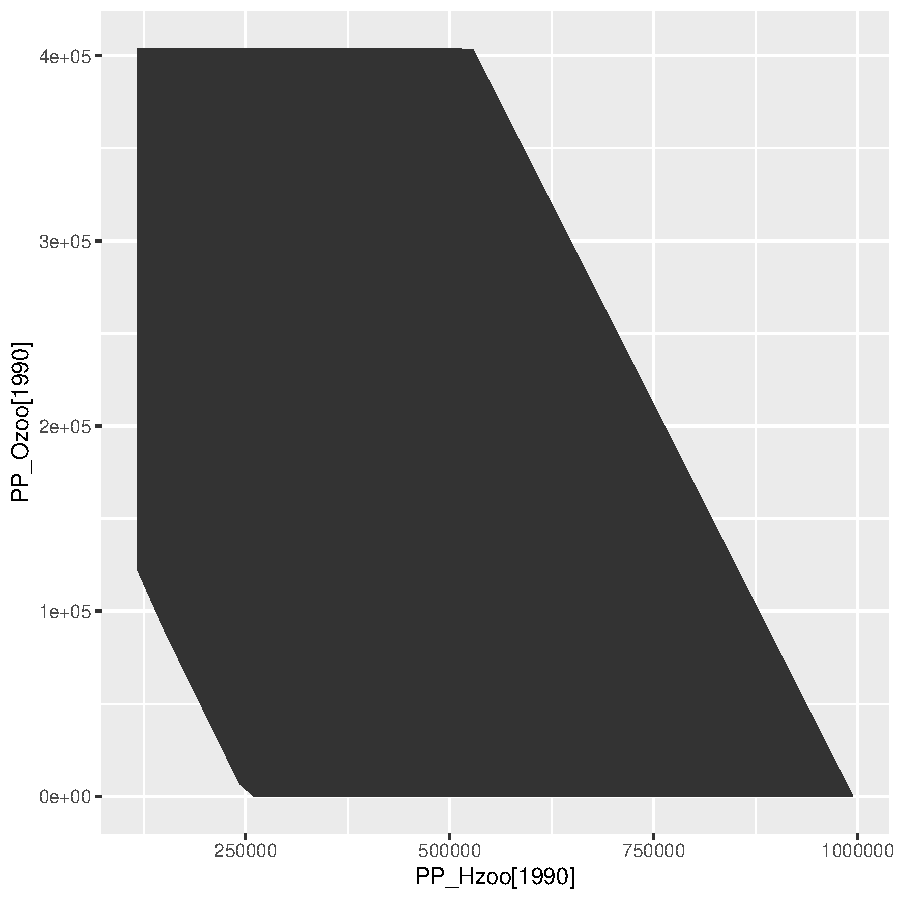
\includegraphics{barents_SM-011}

\clearpage

\section{Sampling polytope}

\subsection{Sampling}

\begin{Schunk}
\begin{Sinput}
> begin = Sys.time()
> SAMPLE <- sampleCaN(POLYTOPE, 
+                       N=100,thin=100, 
+                       nchain=2,
+                       ncore=2)
> end=Sys.time()
> end-begin
\end{Sinput}
\begin{Soutput}
Time difference of 6.5403 secs
\end{Soutput}
\end{Schunk}


\clearpage

\subsection{Convergence}

\begin{Schunk}
\begin{Sinput}
> nchain(SAMPLE$mcmc)
\end{Sinput}
\begin{Soutput}
[1] 2
\end{Soutput}
\begin{Sinput}
> # summary(SAMPLE$mcmc)
\end{Sinput}
\end{Schunk}

Gelman diagnostics

\begin{Schunk}
\begin{Sinput}
> fluxY <- paste(FLUXES[2,1],'[1990]',sep="")
> gelman.diag(SAMPLE$mcmc[,fluxY])
\end{Sinput}
\begin{Soutput}
Potential scale reduction factors:

     Point est. Upper C.I.
[1,]       1.01       1.07
\end{Soutput}
\end{Schunk}


Autocorrelation function

\begin{Schunk}
\begin{Sinput}
> fluxZ <- paste(FLUXES[3,1],'[1990]',sep="")
> thinned_SAMPLE <- window(SAMPLE$mcmc,thin=2)
> thin(thinned_SAMPLE)
\end{Sinput}
\begin{Soutput}
[1] 2
\end{Soutput}
\begin{Sinput}
> acfplot(thinned_SAMPLE[,fluxZ])
\end{Sinput}
\end{Schunk}
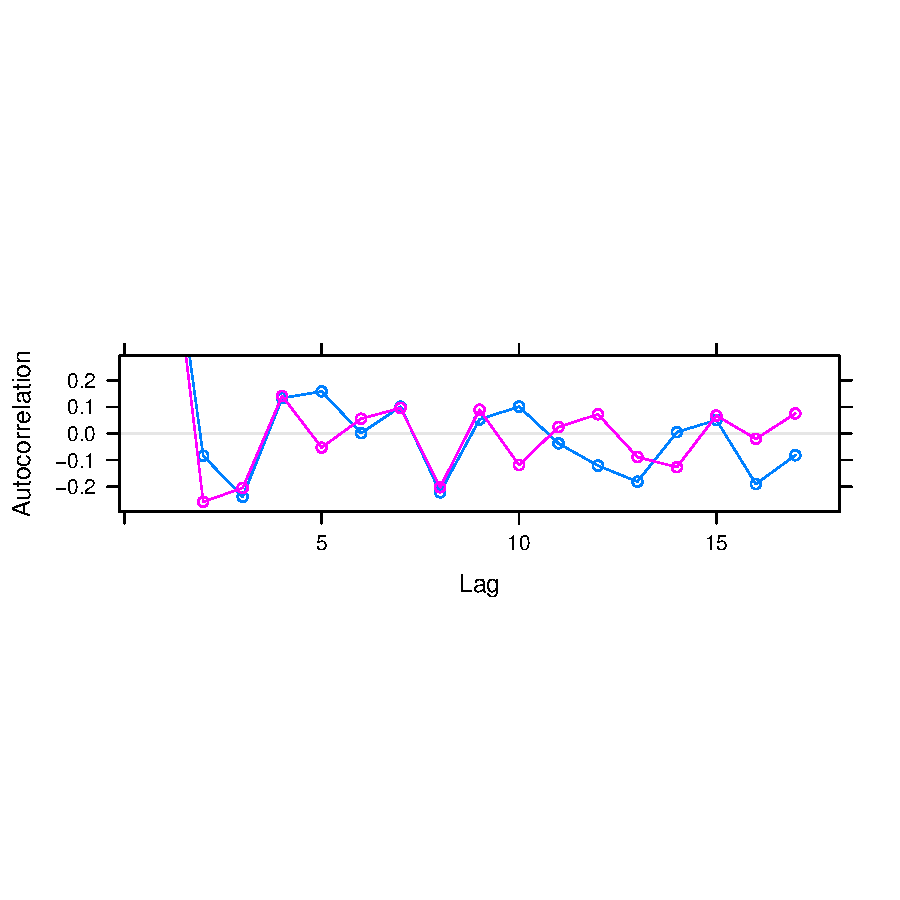
\includegraphics{barents_SM-015}

\clearpage

\subsection{Dynamics}

For several variables or flux, plots of sampled dynamics. 
\begin{Schunk}
\begin{Sinput}
> fluxX <- FLUXES[1,1]
> fluxY <- FLUXES[2,1]
> compA <- COMPONENTS[2,1] 
> compB <- COMPONENTS[3,1] 
> c(fluxX,fluxY,compA)
\end{Sinput}
\begin{Soutput}
[1] "PhytoAndBacteria_HerbZooplankton" "PhytoAndBacteria_OmniZooplankton"
[3] "HerbZooplankton"                 
\end{Soutput}
\end{Schunk}

\begin{Schunk}
\begin{Sinput}
> g <- ggSeries(SAMPLE, c(fluxX,fluxY,compA), TRUE)
> g + scale_y_log10() + guides(color = FALSE, fill = FALSE)
\end{Sinput}
\end{Schunk}
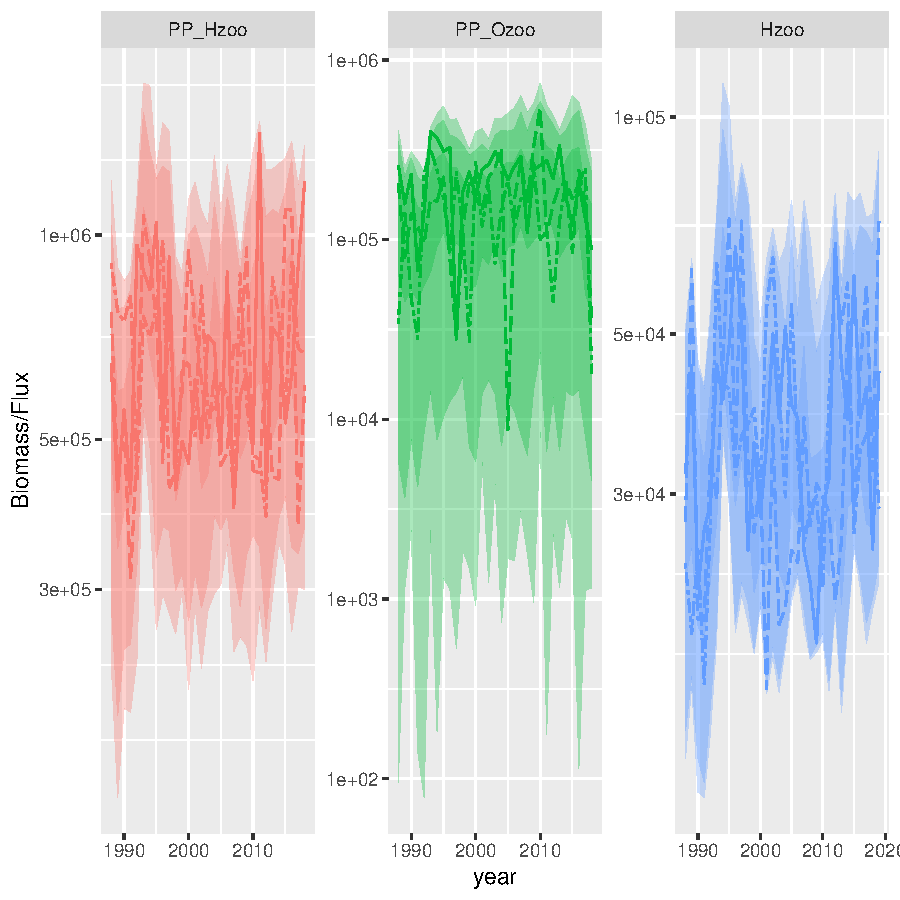
\includegraphics{barents_SM-017}

\clearpage

\subsection{Distribution}

For a component or a flux, for a year, the distribution of sampled values. 
\begin{Schunk}
\begin{Sinput}
> ggViolin(SAMPLE,c(fluxX,fluxY,compA),year=1990,TRUE)
\end{Sinput}
\end{Schunk}
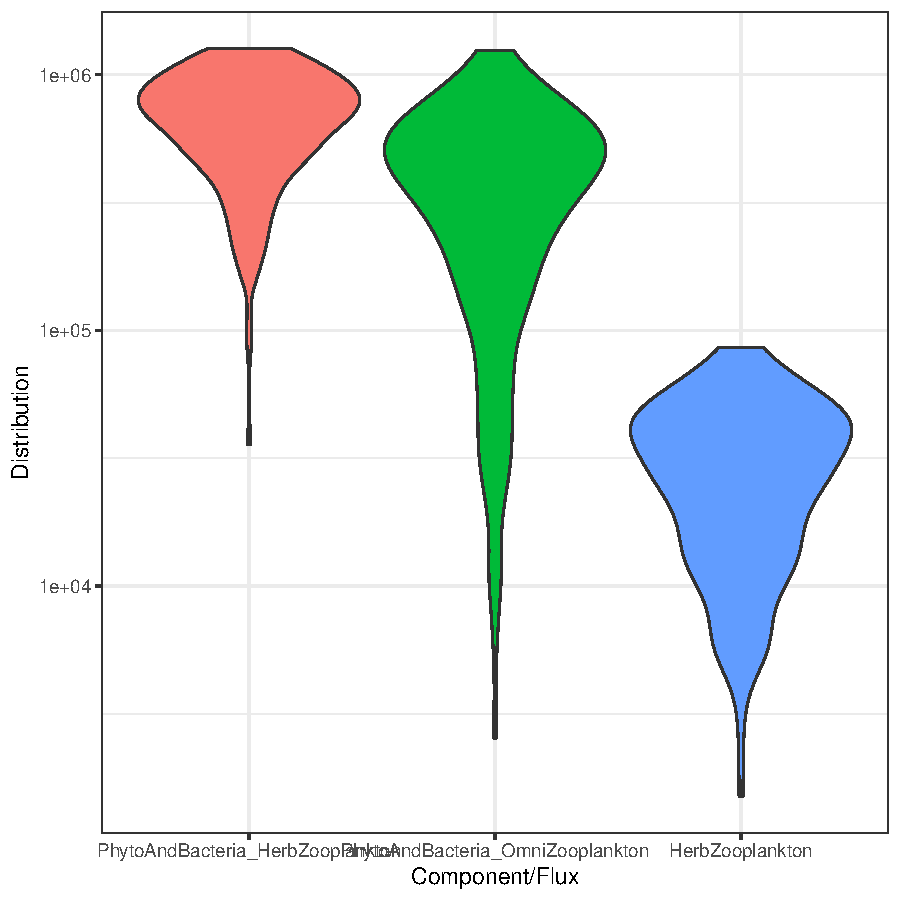
\includegraphics{barents_SM-018}


\clearpage

\subsection{Diet relationships}

\begin{Schunk}
\begin{Sinput}
> ggDiet(SAMPLE, compB)
\end{Sinput}
\end{Schunk}
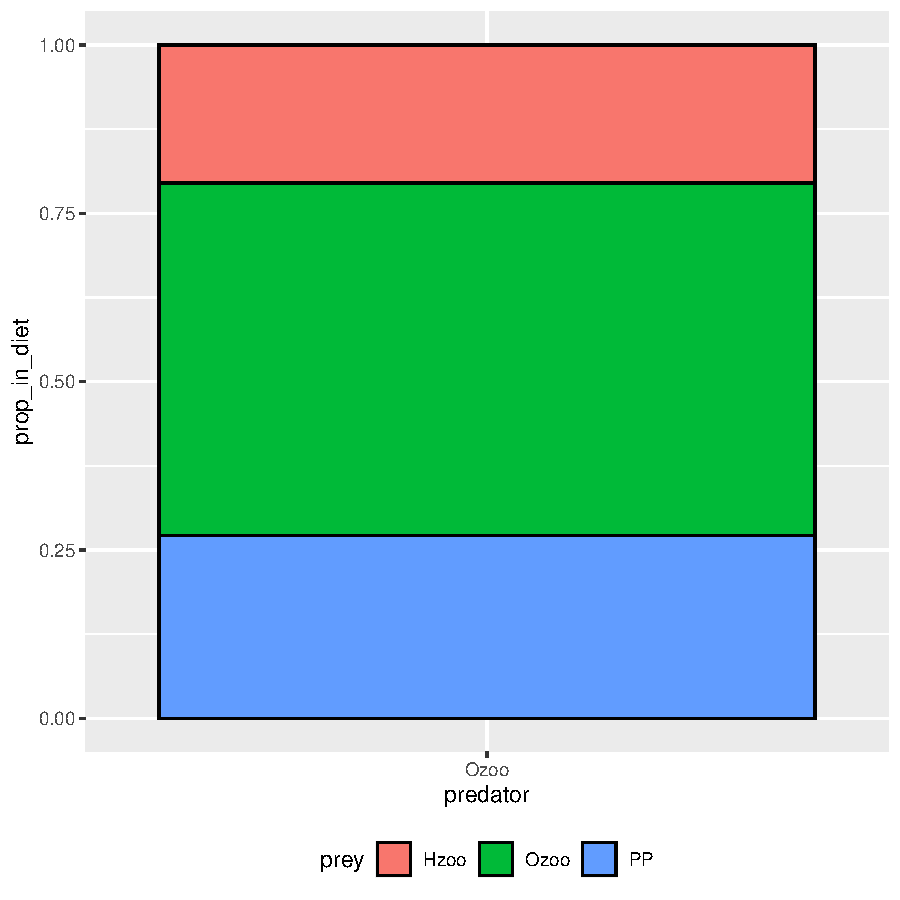
\includegraphics{barents_SM-019}

\subsection{Growth}

\begin{Schunk}
\begin{Sinput}
> ggGrowth(SAMPLE, compB)
\end{Sinput}
\end{Schunk}
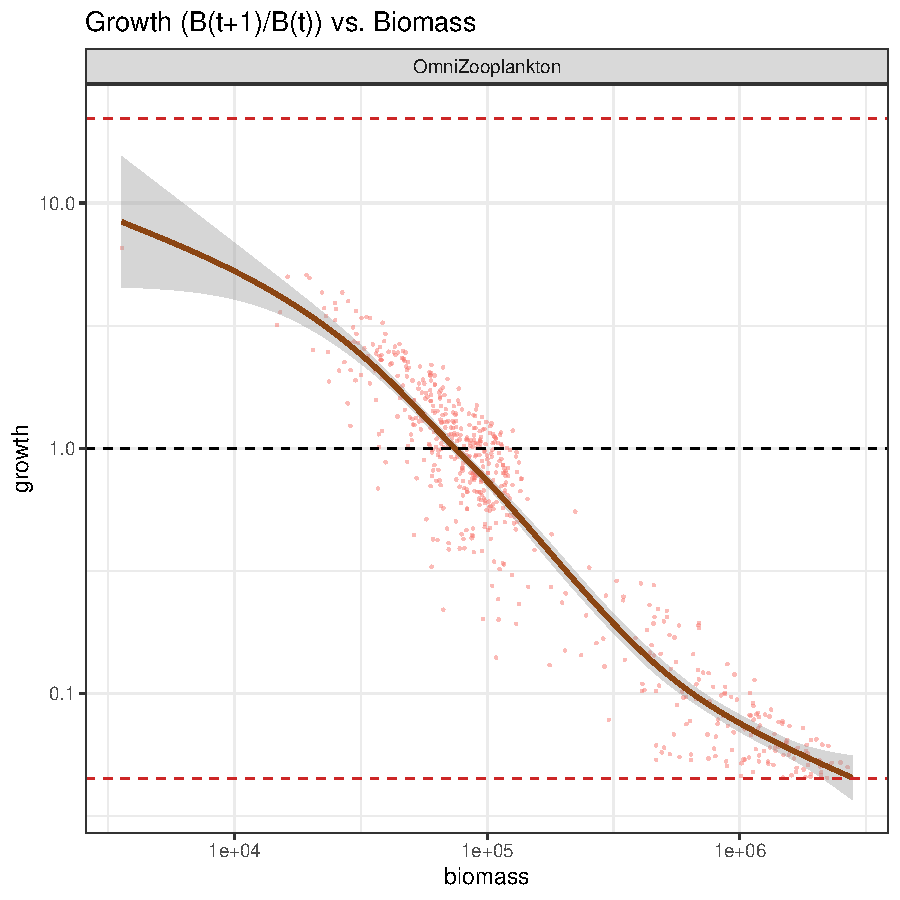
\includegraphics{barents_SM-020}

\subsection{Trophic relation}

\begin{Schunk}
\begin{Sinput}
> ggTrophicRelation(SAMPLE)
> # ggTrophicRelation(SAMPLE, compB)
\end{Sinput}
\end{Schunk}
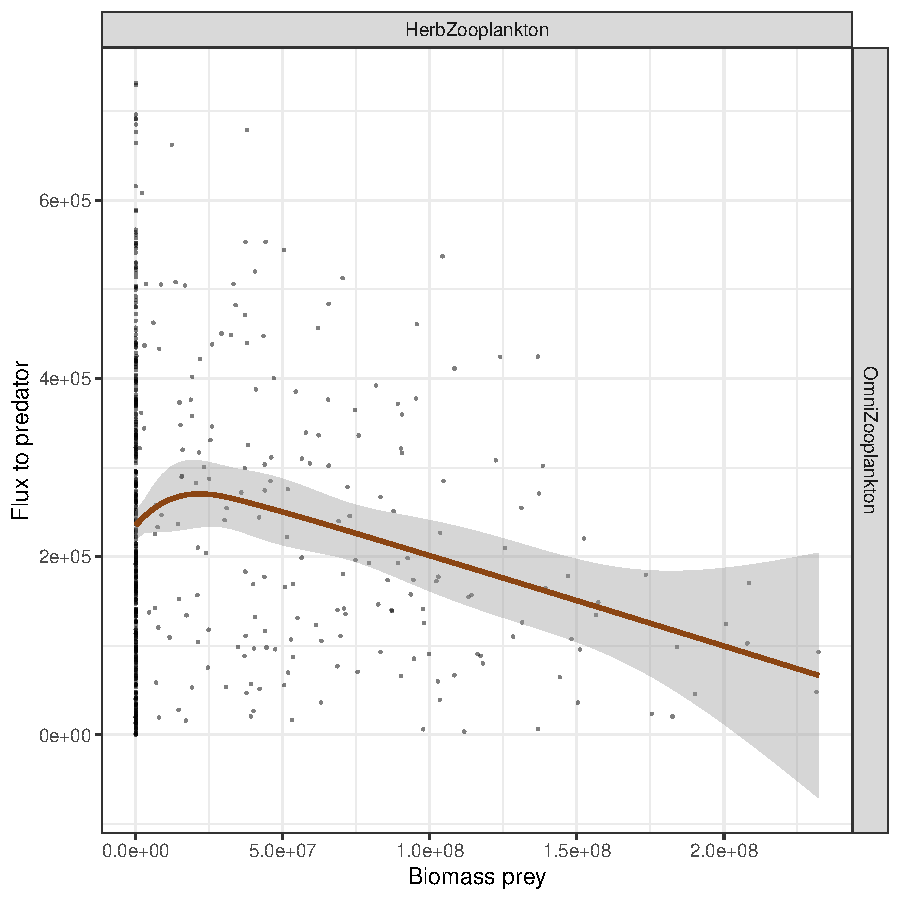
\includegraphics{barents_SM-021}

\subsection{Satiation}

\begin{Schunk}
\begin{Sinput}
> ggSatiation(SAMPLE, compB)
\end{Sinput}
\end{Schunk}
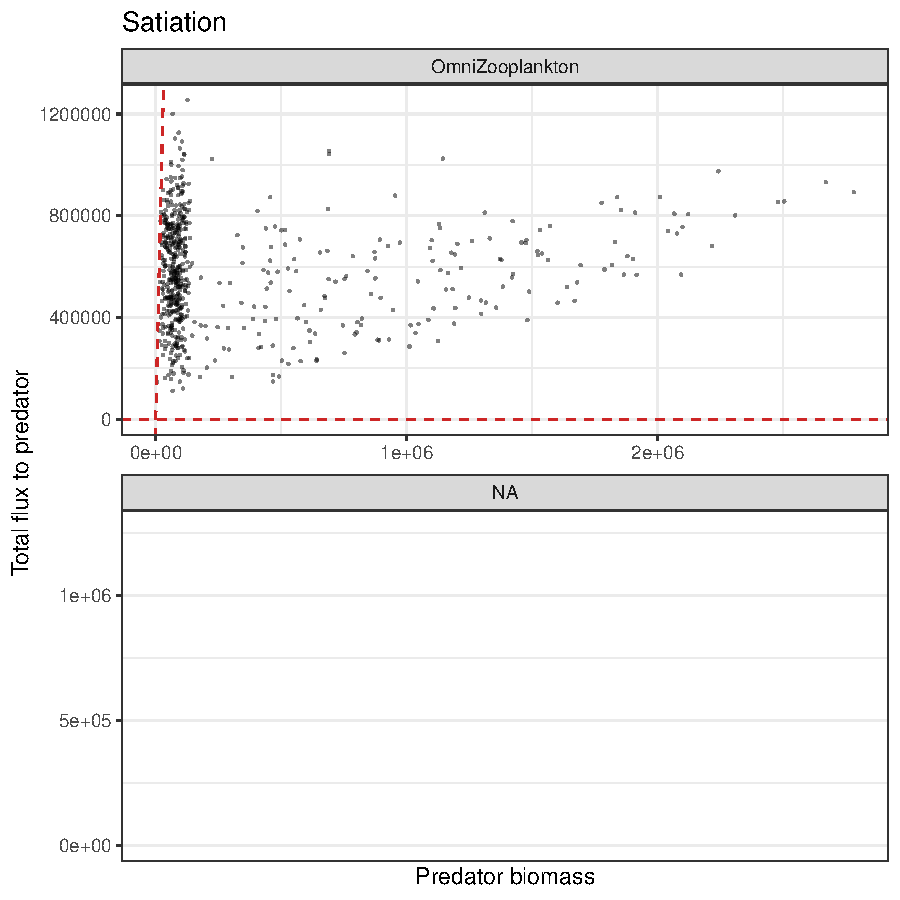
\includegraphics{barents_SM-022}

\section{Try and errors}

\subsection{Activating and desactivating constraint}

\begin{Schunk}
\begin{Sinput}
> #disactivate constraints C02
> constA = CONSTRAINTS[2,1]
> constA
\end{Sinput}
\begin{Soutput}
[1] "C02"
\end{Soutput}
\begin{Sinput}
> POLYTOPEA <- toggleConstraint(POLYTOPE, constA)
\end{Sinput}
\begin{Soutput}
[1] "disactivate inequality C02 : 1988" "disactivate inequality C02 : 1989"
[3] "disactivate inequality C02 : 1990" "disactivate inequality C02 : 1991"
\end{Soutput}
\begin{Sinput}
> #disactivate constraints C02 for year 1991
> constYearA = paste(constA, "1991", sep = " : ")
> POLYTOPEB <- toggleConstraint(POLYTOPE, constYearA)
\end{Sinput}
\begin{Soutput}
[1] "disactivate inequality C02 : 1991"
\end{Soutput}
\end{Schunk}

\begin{Schunk}
\begin{Sinput}
> checkPolytopeStatus(POLYTOPEA)
\end{Sinput}
\begin{Soutput}
[1] "polytope ok"
\end{Soutput}
\begin{Sinput}
> checkPolytopeStatus(POLYTOPEB)
\end{Sinput}
\begin{Soutput}
[1] "polytope ok"
\end{Soutput}
\end{Schunk}

\subsection{Building and analyzing sample}

\begin{Schunk}
\begin{Sinput}
> begin = Sys.time()
> SAMPLEB <- sampleCaN(POLYTOPEB, 
+                       N=100,thin=100, 
+                       nchain=2,
+                       ncore=2)
> end=Sys.time()
> end-begin
\end{Sinput}
\begin{Soutput}
Time difference of 6.61147 secs
\end{Soutput}
\end{Schunk}

\begin{Schunk}
\begin{Sinput}
> fluxX <- FLUXES[1,1]
> fluxY <- FLUXES[2,1]
> compA <- COMPONENTS[2,1] 
> compB <- COMPONENTS[3,1] 
> c(fluxX,fluxY,compA)
\end{Sinput}
\begin{Soutput}
[1] "PhytoAndBacteria_HerbZooplankton" "PhytoAndBacteria_OmniZooplankton"
[3] "HerbZooplankton"                 
\end{Soutput}
\begin{Sinput}
> g <- ggSeries(SAMPLEB, c(fluxX,fluxY,compA), TRUE)
> g + scale_y_log10() + guides(color = FALSE, fill = FALSE)
\end{Sinput}
\end{Schunk}
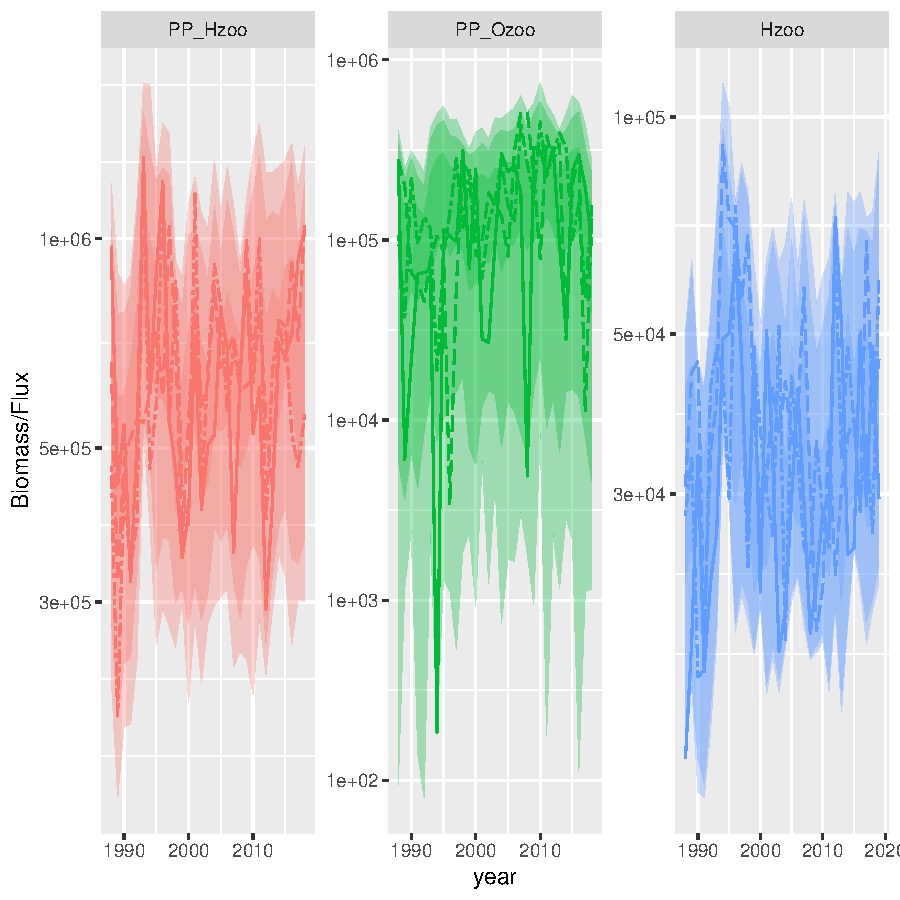
\includegraphics{barents_SM-026}

\end{document}
